\chapter{La rete Tor}
I messaggi trasmessi attraverso l'Onion Routing vengono crittografati a strati con metodi di crittografia simmetrica e inoltrati da dei router o relay, chiamati \emph{Onion Router} ($OR$), in cui � in esecuzione un processo a livello utente, che non necessita di privilegi particolari. Ogni client che vuole stabilire una connessione sicura con un host, deve prima costruire un tunnel attraverso la rete Tor utilizzando un particolare protocollo. Viene detta crittografia stratificata perch� man mano che il messaggio avanza nel tunnel, viene rimosso un livello crittografico, come spiegato nella Figura~\ref{FIG:strat}. Gli utenti che vogliono collegarsi alla rete devono utilizzare un software chiamato \emph{Onion Proxy} ($OP$) che stabilisce i circuiti all'interno della rete e gestisce le connessioni. Ogni router possiede una chiave a lungo termine, utilizzata per firmare i certificati TLS e le proprie caratteristiche che vengono divulgate pubblicamente (come bitrate, indirizzo, tipo ecc.). Inoltre possiede una chiave pubblica a breve termine o onion key usata dai client per crittografare le richieste che, come gi� detto, viene cambiata periodicamente. 

\subsubsection{Le cell}
La maggior parte dei dati scambiati tra due router o tra un router e un client avviene attraverso delle \emph{cell} di dimensione fissa. Esse sono dei pacchetti a livello di applicazione di dimensione fissa di 512 byte, formate da un header e da un payload. L'header contiene informazioni come il circID che serve per identificare il circuito al quale la cell � destinata o anche il CMD che indica cosa fare con il payload. Tutte le comunicazioni router-router e router-client avvengono attraverso delle connessioni TLS (pi� circuiti possono essere multiplati attraverso una connessione TLS). Esistono vari comandi che vengono inseriti nel campo CMD di una cell, ad esempio {\ttfamily CREATE} o {\ttfamily CREATED} usati per costruire un nuovo circuito, oppure {\ttfamily RELAY} che indica che la cell deve essere solo inoltrata al prossimo nodo ecc. Le cell di tipo  {\ttfamily RELAY} possiedono dei campi aggiuntivi all'interno dell'header come lo StreamID che identifica lo stream tra tutti quelli multiplati nel circuito oppure il Digest che serve per verificare l'integrit� dei dati.
\begin{figure}[!htbp]
\centering
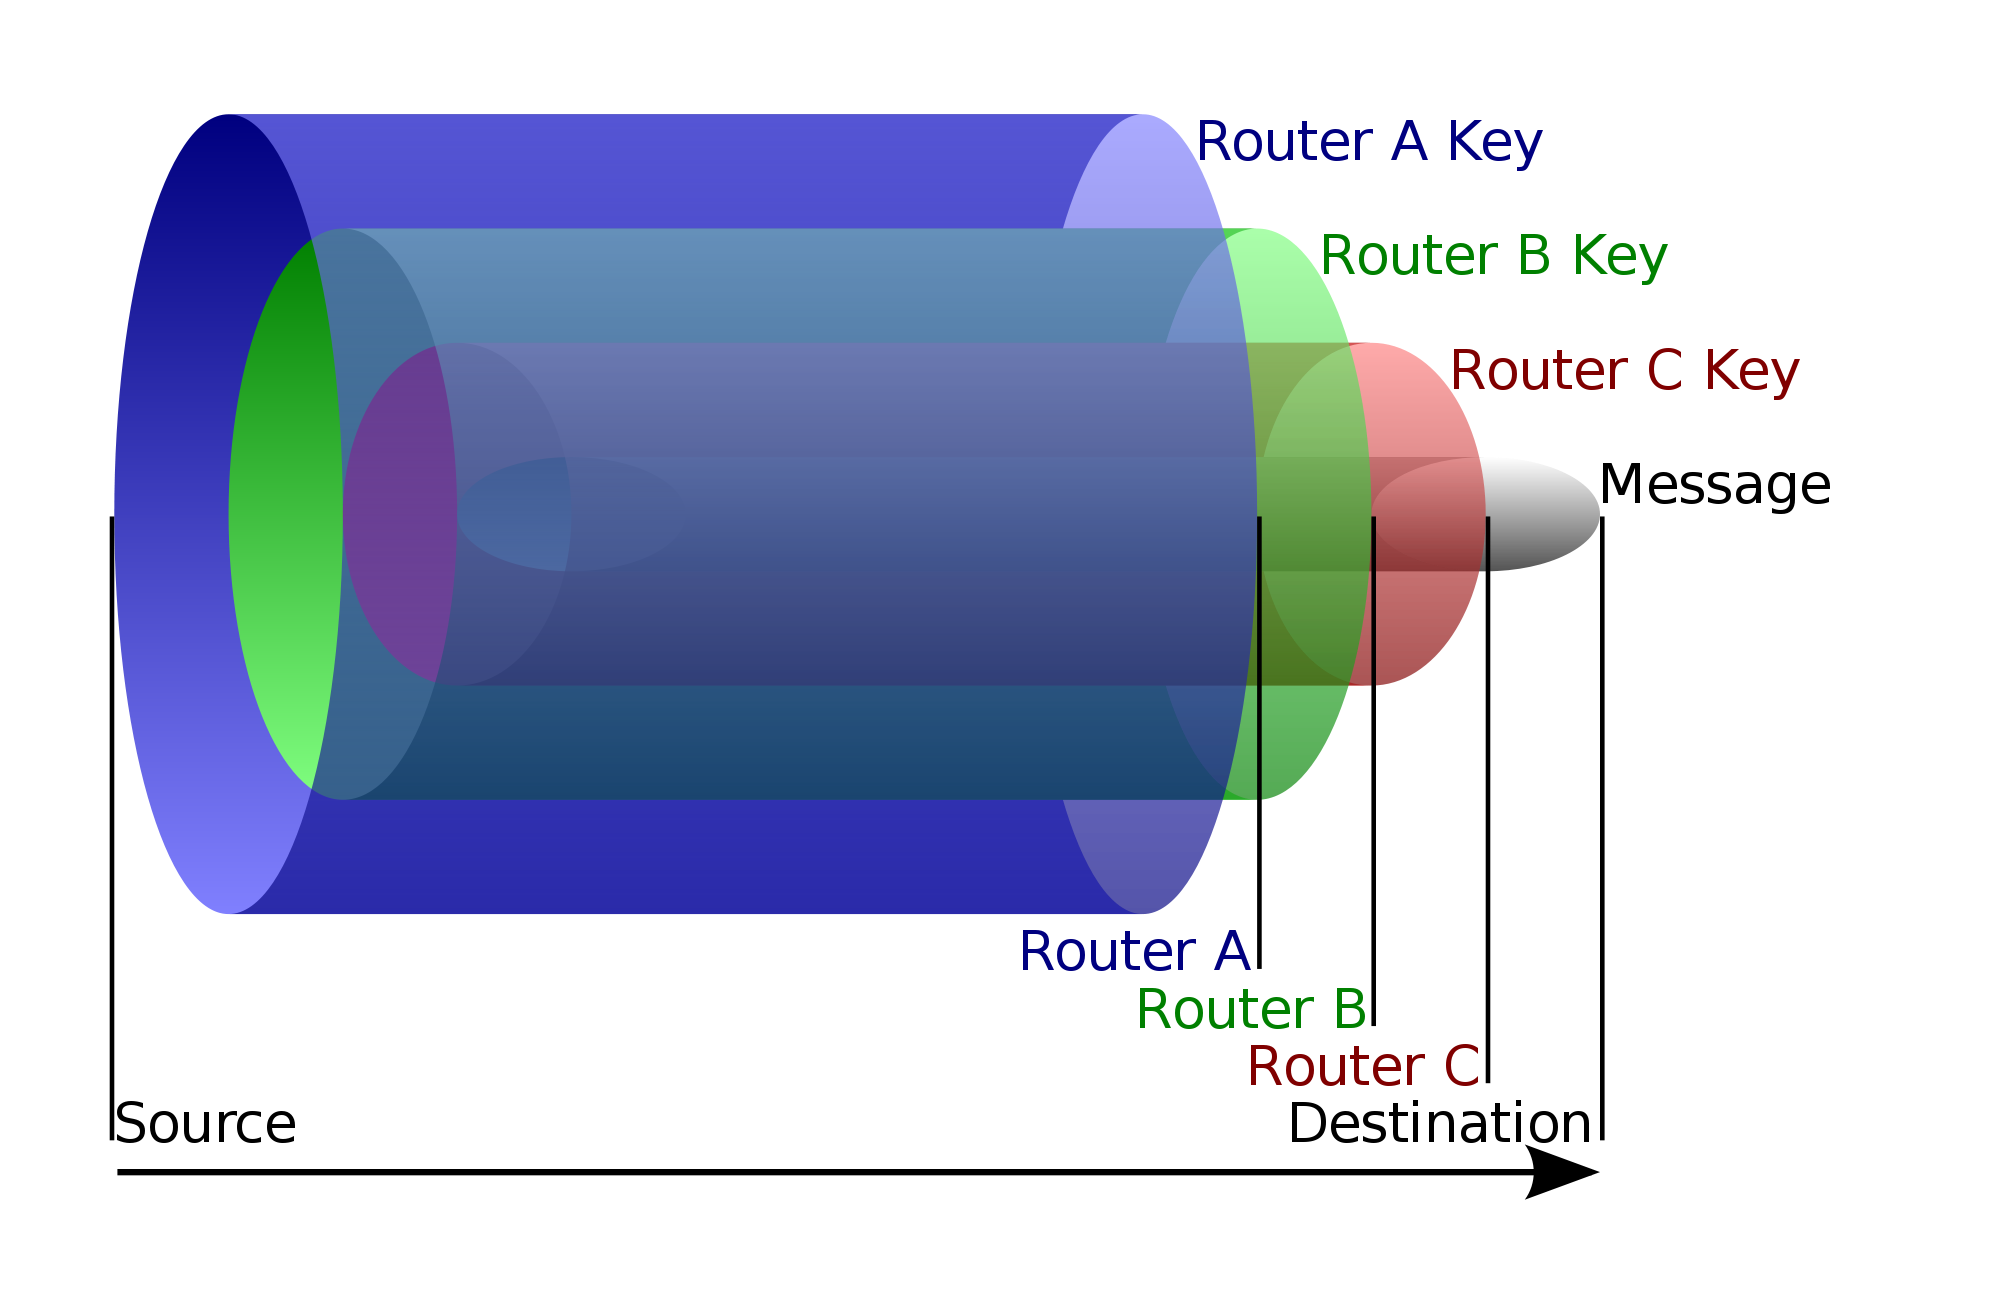
\includegraphics[width=0.5\textwidth]{./figure//strat}
\caption{Livelli di crittografia dell'onion routing.}
\label{FIG:strat}
\end{figure}

\section{Scelta dei nodi e costruzione del circuito}
\begin{figure}[!htbp]
\centering
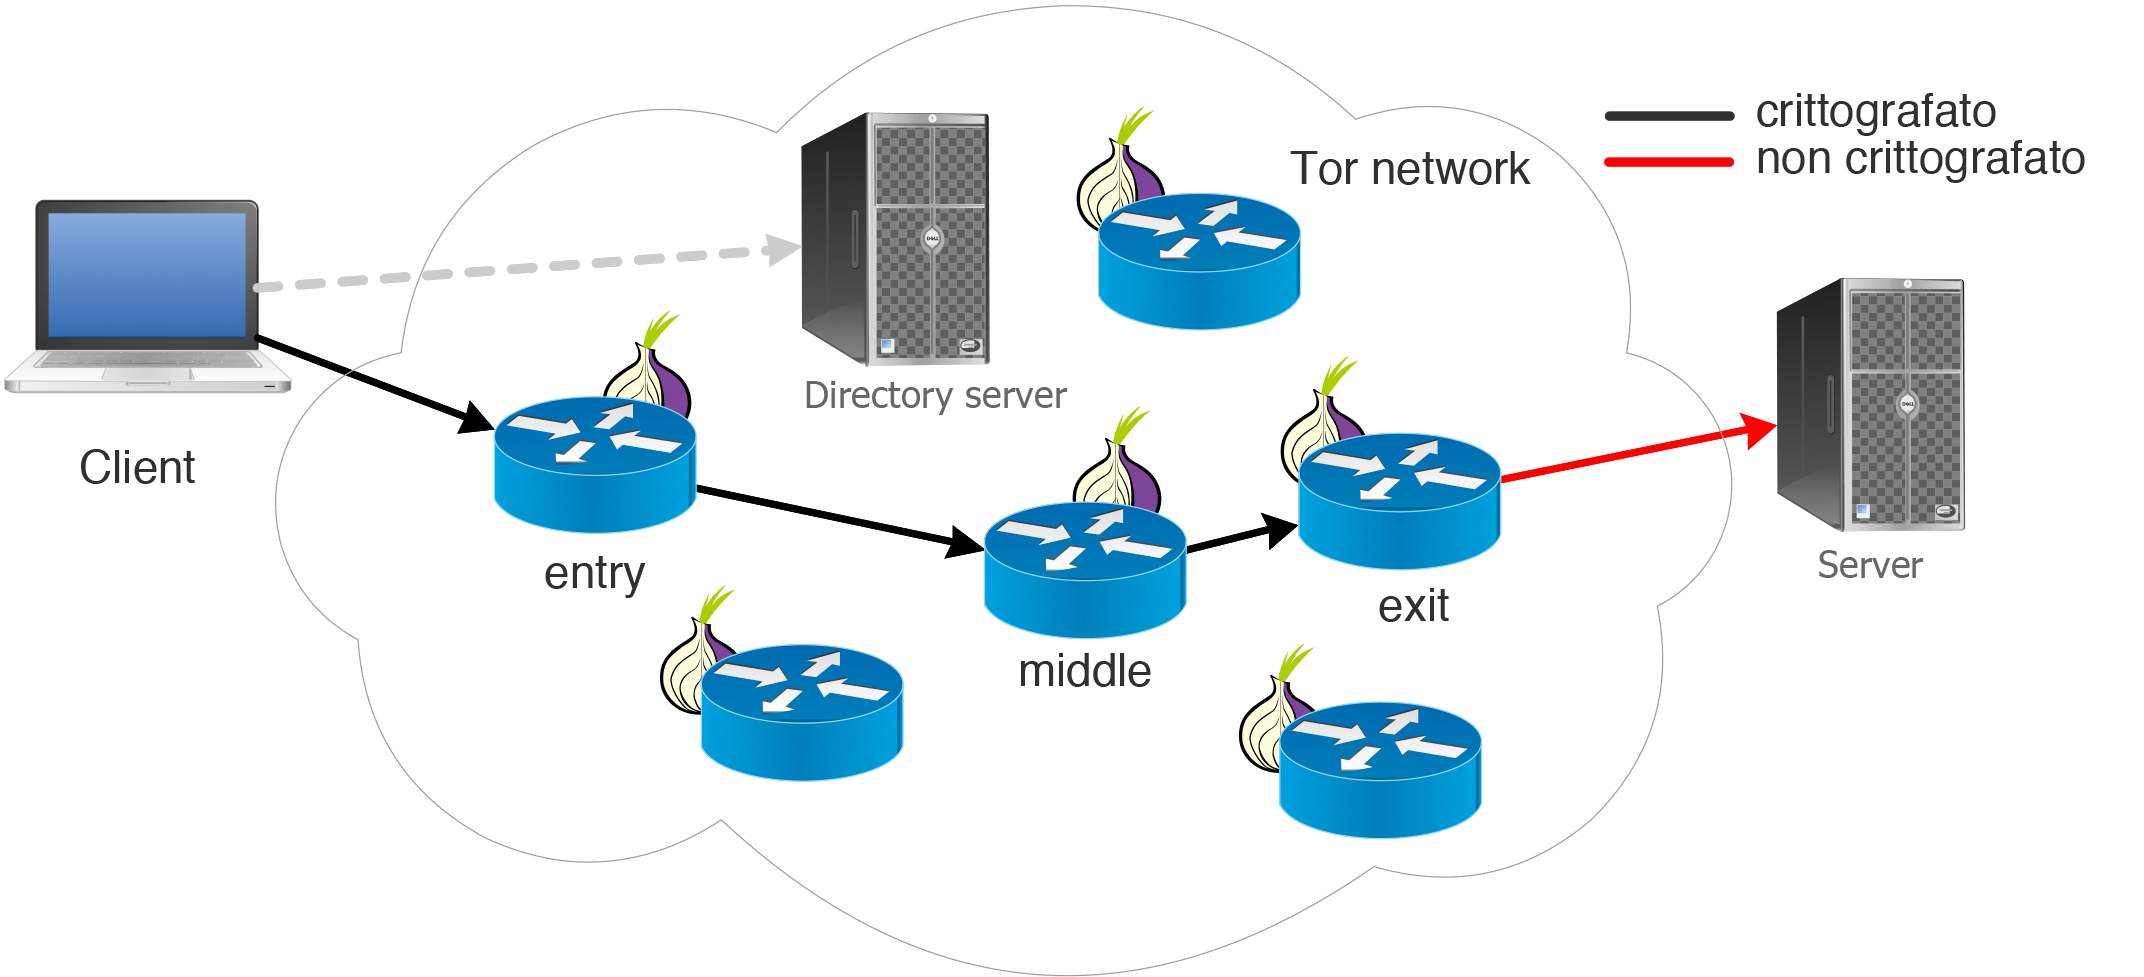
\includegraphics[width=0.7\textwidth]{./figure//tor}
\caption{Circuito Tor.}
\label{FIG:torcirc}
\end{figure}
L'Onion Proxy costruisce in maniera incrementale il circuito, scegliendo solitamente tre Onion Router tra tutti quelli disponibili. Per sapere quali relay sono disponibili in un dato momento, esistono dei \emph{directory server} che contengono una lista di tutti gli $OR$, comprensiva di indirizzo IP, bitrate offerto, chiave pubblica e altre informazioni. Come mostrato in Figura~\ref{FIG:torcirc} ogni circuito � costituito da un entry router, un middle e un exit. Per assicurare buone prestazioni essi vengono scelti tramite un algoritmo pesato di selezione che tiene conto del bitrate che ogni router annuncia.
I router possono essere suddivisi in quattro insiemi diversi: pure entry (o entry guard) ($G_{0}$), pure exit ($E_{0}$), sia entry che exit ($A$) e n� entry n� exit ($N_E$). 
Indichiamo con $i$ l' i-esimo router all'interno della rete con $i=1,2,...,N$ dove $N$ � il numero totale di onion router. Possiamo dare quindi le seguenti definizioni:
\begin{equation}
E_{0}=\{i: OR_{i} \, \text{� pure exit}\} \subset E \text{ con } E=\{i: OR_{i} \, \text{� exit}\} \subset \{\text{$1$, $2$,...,$N$}\} 
\end{equation}

\begin{equation}
 G_{0}=\{i: OR_{i} \, \text{� pure entry}\} \subset G \text{ con } G=\{i: OR_{i} \, \text{� entry}\} \subset \{\text{$1$, $2$,...,$N$}\}.
\end{equation}
 Da cui derivano le relazioni:
\begin{equation}
E=A \cup E_{0} \text{ e } G=A \cup G_{0}
\end{equation}
che indicano che gli entry router sono formati dall'unione dei pure entry e da quelli che possono operare sia da entry che da exit; la stessa cosa vale per gli exit.
Se $B_{i}$ rappresenta il bitrate dell' i-esimo router (uguale sia in ingresso che in uscita), il bitrate totale della rete sar� definita come:
\begin{equation}
B=\sum_{i=1}^N B_{i}
\end{equation}
mentre il bitrate totale di uscita, puramente di uscita, di ingresso e puramente di ingresso sono rispettivamente:
\[
B_{E}=\sum_{i\in E}B_{i} \text{ , } B_{E_0}=\sum_{i\in E_0}B_{i} \text{ , } B_{G}=\sum_{i\in G}B_{i} \text{ , } B_{G_0}=\sum_{i\in G_0}B_{i} \text{.}
\]
Per primo viene scelto il router di uscita e quindi bisogna definire un peso per il bitrate dei router $\in A$ (in quanto anche essi possono essere scelti come exit):

\begin{equation}
\label{eqn:wgpath}
W_G=
\begin{cases}
1-\frac{B}{3B_G},      	& \text{$altrimenti$,} \\
0, 									& \text{se $B_G < B/3$.}
\end{cases}
\end{equation}
Allora la probabilit� di scegliere l' i-esimo router, come router di uscita � definita come:

\begin{equation}
P_i=
\begin{cases}
\frac{B_i}{B_{E_{0}}+W_G B_A},      	& i \in E_0 \\
\frac{W_G B_i}{B_{E_{0}}+W_G B_A}, 	& i \in A.
\end{cases}
\end{equation}
Questo significa che, se ad esempio, il bitrate in ingresso � scarso ($B_G < B/3$), i router che possono operare sia da entry che da exit, non verranno considerati nel momento in cui verr� scelto il nodo di uscita. Per la scelta del router d'ingresso vale lo stesso ragionamento:

\begin{equation}
\label{eqn:wepath}
W_E=
\begin{cases}
1-\frac{B}{3B_E},      	& \text{$altrimenti$,} \\
0, 									& \text{se $B_E < B/3$}
\end{cases}
\end{equation}
e la probabilit� di scegliere un router come entry diventa:

\begin{equation}
P_i=
\begin{cases}
\frac{B_i}{B_{G_{0}}+W_E B_A},      	& i \in G_0 \\
\frac{W_E B_i}{B_{G_{0}}+W_E B_A}, 	& i \in A
\end{cases}
\end{equation}
con $B_{A}=\sum_{i\in A}B_{i}$.
Dopo aver scelto i router di uscita e di ingresso, si procede con la scelta del middle. Anche in questo caso vanno valutati i pesi prima di calcolare la probabilit� che venga scelto l'i-esimo router:

\begin{equation}
\bar{B_{i}} =
\begin{cases}
W_E B_i,      	& i \in E_0 \\
W_G B_i, 	& i \in G_0 \\
W_E W_G B_i, 	& i \in A \\
B_i,	& i \in N_E 
\end{cases}
 \text{ , } 
P_i=\frac{\bar{B_{i}}}{B_{E_{0}}W_{E}+B_{G_{0}}W_{G}+B_{A}W_{E}W_{G}+B_{N}}
\end{equation}
Una volta scelti i nodi che andranno a costituire il circuito, il client (Alice nella Figura~\ref{FIG:circbuild}) invia una {\ttfamily CREATE} cell al router d'ingresso, contenente la prima met� dell'handshake ($g^x$) di Diffie-Hellman, crittografata con l'onion key. L'$OR_{1}$ deve quindi decifrare la richiesta e rispondere con una {\ttfamily CREATED} cell contenente ($g^y$) insieme all'hash della chiave negoziata $K=g^{(xy)}$. Da questo momento in poi Alice e l'entry router potranno comunicare utilizzando un algoritmo di crittografia simmetrica (tipicamente AES) con la chiave appena concordata. Per estendere il circuito, il client deve inviare una {\ttfamily RELAY\textunderscore EXTEND} cell al router d'ingresso, comprensiva dell'indirizzo del prossimo relay e della prima met� della dell'handshake di Diffie-Hellman ($g^{x_{2}}$). L'entry copia il mezzo handshake in una {\ttfamily CREATE} cell e la inoltra al middle router. Quando l'$OR_{2}$ risponde con la {\ttfamily CREATED} cell, l'$OR_{1}$ copia il payload all'interno di una  {\ttfamily RELAY\textunderscore EXTENDED} cell e la invia ad Alice. Adesso anche Alice e il middle router condividono una chiave $K_{2}=g^{(x_{2}y_{2})}$ da utilizzare per comunicare tra di loro. Per estendere ulteriormente il circuito, viene ripetuta la procedura appena descritta, comunicando il comando di estensione all'ultimo router. Normalmente, quando due router o un router e il client devono comunicare tra di loro, utilizzano le {\ttfamily RELAY} cell. Quando il client fa una richiesta, ad esempio ad un server web che si trova al di fuori della rete Tor, essa viene incapsulata in una {\ttfamily RELAY} cell, crittografata sequenzialmente con le chiavi di sessione e inviata all'entry. La cell deve percorrere il circuito dal primo all'ultimo router, ognuno dei quali si occupa di rimuovere un livello di crittografia. L'ultimo router, oltre a rimuovere l'ultimo livello, inoltra la richiesta al server e riceve la risposta. Una volta ricevuta la risposta, anch'essa viene incapsulata in una cell, crittografata con la chiave di sessione e rispedita al nodo precedente, proseguendo allo stesso modo attraverso gli altri nodi. Il nodo di uscita quindi esegue le operazioni per conto del client, aprendo una connessione in genere non crittografata con gli host esterni alla rete Tor. Grazie al meccanismo appena descritto, il client pu� rimanere in totale anonimato, poich� ogni router conosce solo i due nodi con i quali sta comunicando, ma non conosce gli altri componenti del circuito.
\begin{figure}[!htbp]
\centering
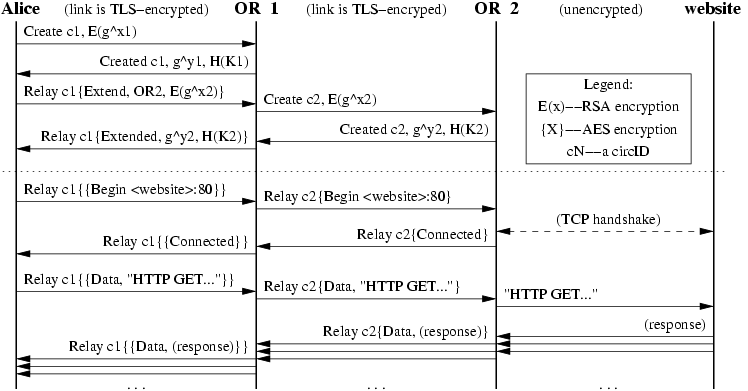
\includegraphics[width=0.9\textwidth]{./figure//circuit-building}
\caption{Procedura per la costruzione di un circuito e richiesta ad un server web.}
\label{FIG:circbuild}
\end{figure}

\newpage
\section{Servizi Nascosti}
Oltre a garantire l'anonimato ai client, Tor � in grado di fare la stessa cosa lato server. Questo significa che � possibile fornire un servizio (come ad esempio un sito web), facendo in modo che la localizzazione del server rimanga sconosciuta. Per accedere ad un servizio nascosto, un client deve obbligatoriamente utilizzare Tor, e deve riferirsi ad esso attraverso un pseudo dominio di primo livello ".onion". Quando un nuovo servizio viene attivato, esso deve comunicare la propria esistenza alla rete per poter essere raggiungibile dai client. Per prima cosa deve stabilire dei \emph{punti di introduzione}, cio� scegliere in maniera casuale dei router e costruire dei circuiti che terminano in questi ultimi, comunicandogli di rimanere in attesa di richieste. Successivamente viene inviato ad un database, un \emph{descrittore} (firmato con la chiave privata), contenente la chiave pubblica e un elenco dei punti di introduzione.\\ Quando un client (Alice) tenta di contattare un servizio nascosto (Bob), vengono eseguite le seguenti operazioni:
\begin{enumerate}
\item Alice esegue una chiamata all'indirizzo xyz.onion, per ottenere il descrittore del servizio e conoscere cos� i suoi punti di introduzione (xyz � una sequenza di 16 caratteri derivante dalla chiave pubblica del servizio stesso); 
\item Alice sceglie un $OR$ come \emph{punto di rendezvous}  da utilizzare per connettersi al servizio;
\item  Alice apre un circuito anonimo con uno dei punti di introduzione per comunicare al servizio il punto di rendezvous scelto e la prima met� dell'handshake di DH;
\item se Bob accetta la richiesta, si connette al punto di rendezvous e comunica ad Alice la seconda met� dell'handshake di DH e un hash della chiave concordata;
 \item adesso il punto di rendezvous collega il circuito di Alice con quello di Bob, che potranno comunicare in maniera del tutto anonima.
\end{enumerate}



%\begin{enumerate}
%\item eseguire una chi
%\end{enumerate}

%\lipsum[1-2]
%%%%% authority tor


% ---------------------  ESEMPI UTILI PRONTI ALL'USO  ----------------------------
%TERZO capitolo della tesi. Esempio di citazione doppia \cite{Munoz-Lipo,Vas}.
%
%Esempio di figura in \figurename\ \ref{FIG:LogoUniPD}.
%
%\begin{figure}[!htbp]
%\centering
%
\includegraphics[width=0.25\textwidth]{./figure//LogoUniPD}
%\caption{Esempio di figura.}
%\label{FIG:LogoUniPD}
%\end{figure}
%
%Esempio di tabella in \tablename\ \ref{TAB:Esempio}.
%
%\begin{table}[!htbp]
%\centering
%\renewcommand{\arraystretch}{1.3}
%\caption{Esempio di tabella.}
%\begin{tabular}{cc}
%\hline
%Nome & Valore \\
%\hline
%a & 1 \\
%b & 2 \\
%c & 3 \\
%d & 4 \\
%e & 5 \\
%f & 6 \\
%\hline
%\end{tabular}
%\label{TAB:Esempio}
%\end{table}